\documentclass{article}
\usepackage{graphicx} % Required for inserting images
% Useful packages for computer science thesis
\usepackage{amsmath}  % Advanced math formatting
\usepackage{amsthm}   % Theorem environments
\usepackage{algorithmic}  % Algorithm writing
\usepackage{algorithm}    % Algorithm floating environment
\usepackage{listings}     % Code listings
\usepackage{xcolor}       % Color support
\usepackage{caption}
\usepackage{multirow}
\usepackage{tikz}
\usepackage{amssymb}
\usepackage{booktabs}
\usepackage{makecell}
\usepackage{subcaption}
\usepackage{booktabs}     % Professional tables
\usepackage{hyperref}     % PDF bookmarks and hyperlinks
\usepackage{cleveref}     % Smart cross-referencing
\usepackage{url}          % URL formatting

% Configure hyperref
\hypersetup{
    colorlinks=true,
    linkcolor=black,
    filecolor=magenta,
    urlcolor=[rgb]{0.0, 0.3, 0.7},
    citecolor=[rgb]{0.0, 0.5, 0.0}
}


\title{Second Assignment}
\author{Andrea Lavino}
\date{March 2025}

\begin{document}

\maketitle

\clearpage

\tableofcontents

\clearpage

% --- Very Busy Expressions --- %
\section{Very Busy Expressions}

The search for very busy expressions can be useful for code hoisting, since very busy expressions can be moved from the place they are up to a joint point from which the flow departures.

\subsection{Problem formalization}

Formally an expression is said to be \textbf{very busy} when it is computed along each path that part from the point \textit{p} without any redefinition of its operands. This information can be used to move the expression to a point of the code in which is computation can be used by all the paths that use the expression.

\begin{table}[H]
	\centering
	\begin{tabular}{|p{0.4\textwidth}|p{0.4\textwidth}|}
		\hline
		                          & \textbf{Very Busy Expressions}     \\
		\hline
		Domain                    & Sets of expressions                \\
		\hline
		Direction                 & Backward                           \\
		                          & $in[b] = f_b(out[b])$              \\
		                          & $out[b] = \wedge in[succ(b)]$      \\
		\hline
		Transfer function         & $f_b(x) = Gen_b \cup (x - Kill_b)$ \\
		\hline
		Meet Operation ($\wedge$) & $\cap$                             \\
		\hline
		Boundary Condition        & $out[exit] = \varnothing$          \\
		\hline
		Initial interior points   & $out[b] = U$                       \\
		\hline
	\end{tabular}
	\caption{Very busy expressions summary table}
	\label{tab:dataflow_problem_x}
\end{table}

\subsection{Example}

\begin{figure}[H]
	\centering
	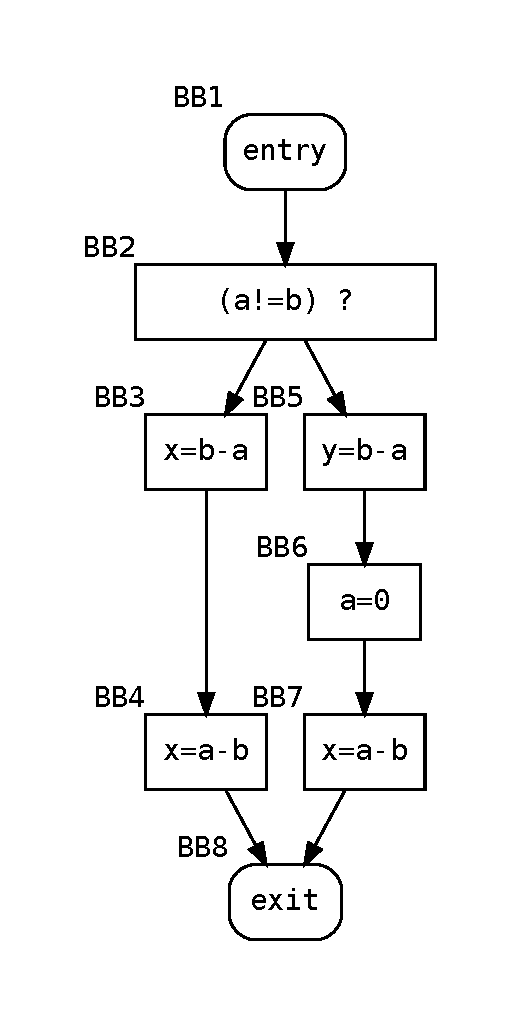
\includegraphics[width=0.4\textwidth]{graphs/very_busy.pdf}
	\caption{Very Busy Expression Example}
	\label{fig:very-busy}
\end{figure}

\begin{table}[H]
	\centering
	\begin{tabular}{|c|c|c|c|c|}
		\hline
		             & \multicolumn{2}{c|}{\textbf{Iteration 1}} & \multicolumn{2}{c|}{\textbf{Iteration 2}}                                        \\ \hline
		             & \textbf{IN[B]}                            & \textbf{OUT[B]}                           & \textbf{IN[B]}     & \textbf{OUT[B]} \\ \hline
		\textbf{BB1} & $\{b-a\}$                                 & $\{b-a\}$                                 & $\{b-a\}$          & $\{b-a\}$       \\ \hline
		\textbf{BB2} & $\{b-a\}$                                 & $\{b-a\}$                                 & $\{b-a\}$          & $\{b-a\}$       \\ \hline
		\textbf{BB3} & $\{b-a\}, \{a-b\}$                        & $\{a-b\}$                                 & $\{b-a\}, \{a-b\}$ & $\{a-b\}$       \\ \hline
		\textbf{BB4} & $\{a-b\}$                                 & $\varnothing$                             & $\{a-b\}$          & $\varnothing$   \\ \hline
		\textbf{BB5} & $\{b - a\}$                               & $\varnothing$                             & $\{b - a\}$        & $\varnothing$   \\ \hline
		\textbf{BB6} & $\varnothing$                             & $\{a-b\}$                                 & $\varnothing$      & $\{a-b\}$       \\ \hline
		\textbf{BB7} & $\{a-b\}$                                 & $\varnothing$                             & $\{a-b\}$          & $\varnothing$   \\ \hline
		\textbf{BB8} & $\varnothing$                             & $\varnothing$                             & $\varnothing$      & $\varnothing$   \\ \hline
	\end{tabular}
	\caption{Very Busy Expression Algorithm Execution Table}
\end{table}

% --- Dominator Analysis --- %
\section{Dominator Analysis}

Dominator analysis is fundamental to create the single static assignment form.

\subsection{Problem formalization}

A basic block $B_1$ \textbf{dominates} another block $B_2$ if it is encountered in every path from entry to $B_2$.

\begin{table}[H]
	\centering
	\begin{tabular}{|p{0.4\textwidth}|p{0.45\textwidth}|}
		\hline
		                          & \textbf{Dominator Analysis}                                                             \\
		\hline
		Domain                    & Sets of Basic Blocks                                                                    \\
		\hline
		Direction                 & Forward                                                                                 \\
		\hline
		Transfer function         & $f_b(x) = \{x\} \cup (\bigcap_{m \in preds(x)} f_b(m)) $                                \\
		\hline
		Meet Operation ($\wedge$) & $\cap$                                                                                  \\
		\hline
		Boundary Condition        & $Dom[entry] = \{entry\}$                                                                \\
		\hline
		Initial interior points   & $Dom[b] = N \quad \forall b \neq entry$, with $N$ the number of basic blocks of the CFG \\
		\hline
	\end{tabular}
	\caption{Dataflow Problem X Properties}
	\label{tab:dataflow_problem_x}
\end{table}

\subsection{Example}

\begin{figure}[H]
	\centering
	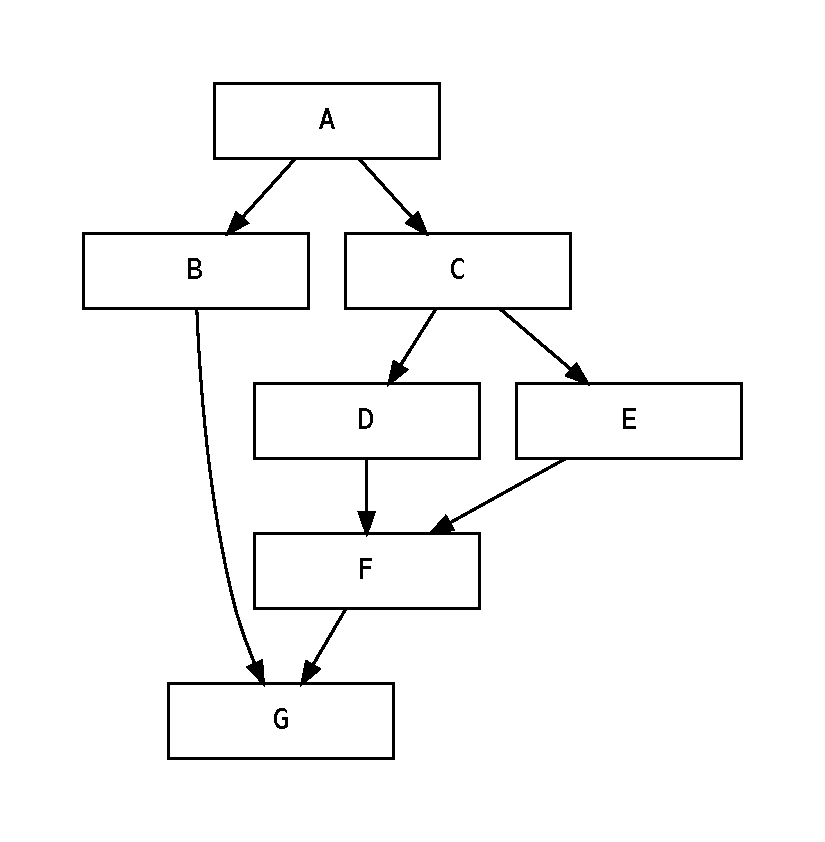
\includegraphics[width=0.5\textwidth]{graphs/dominance.pdf}
	\caption{Dominance Analysis example}
	\label{fig:enter-label}
\end{figure}

\begin{table}[H]
	\centering
	\begin{tabular}{|c|c|c|c|c|c|c|}
		\hline
		           & \textbf{DOM[B]} \\ \hline
		\textbf{A} & $\{A\}$         \\ \hline
		\textbf{B} & $\{A, B\}$      \\ \hline
		\textbf{C} & $\{A, C\}$      \\ \hline
		\textbf{D} & $\{A, C, D\}$   \\ \hline
		\textbf{E} & $\{A, C, E\}$   \\ \hline
		\textbf{F} & $\{A, C, F\}$   \\ \hline
		\textbf{G} & $\{A, G\}$      \\ \hline
	\end{tabular}
	\caption{Dominance analysis execution table}
\end{table}

% --- Constant Propagation --- %
\section{Constant Propagation}

The constant propagation problem aims at finding what are the couples $<variable, constant \ value>$ that are availables in a certain basic block, so that the variable constant value can be propagated across the blocks.

\subsection{Problem formalization}

We say that a couple $<variable, constant>$ is valid at block $n$ if it is guaranteed that the variable $x$ gets that constant value every time that the block is reached.

\begin{table}[H]
	\centering
	\begin{tabular}{|p{0.4\textwidth}|p{0.4\textwidth}|}
		\hline
		                          & \textbf{Constant Propagation}                            \\
		\hline
		Domain                    & Sets of variables and their constant values              \\
		\hline
		Direction                 & Forward                                                  \\
		                          & $in[b] = \wedge(out[pred(b)])$                           \\
		                          & $out[b] = f_b(in[b])$                                    \\
		\hline
		Transfer function         & $f_b(x) = Gen_b \cup (x - Kill_b)$                       \\
		\hline
		Meet Operation ($\wedge$) & $\cap$                                                   \\
		\hline
		Boundary Condition        & $out[entry] = \varnothing \quad in[entry] = \varnothing$ \\
		\hline
		Initial interior points   & $out[b] = \varnothing \quad in[b] = U$                   \\
		\hline
	\end{tabular}
	\caption{Constant Propagation Problem Summary Table}
	\label{tab:dataflow_problem_x}
\end{table}

\subsection{Example}

\begin{figure}[H]
	\centering
	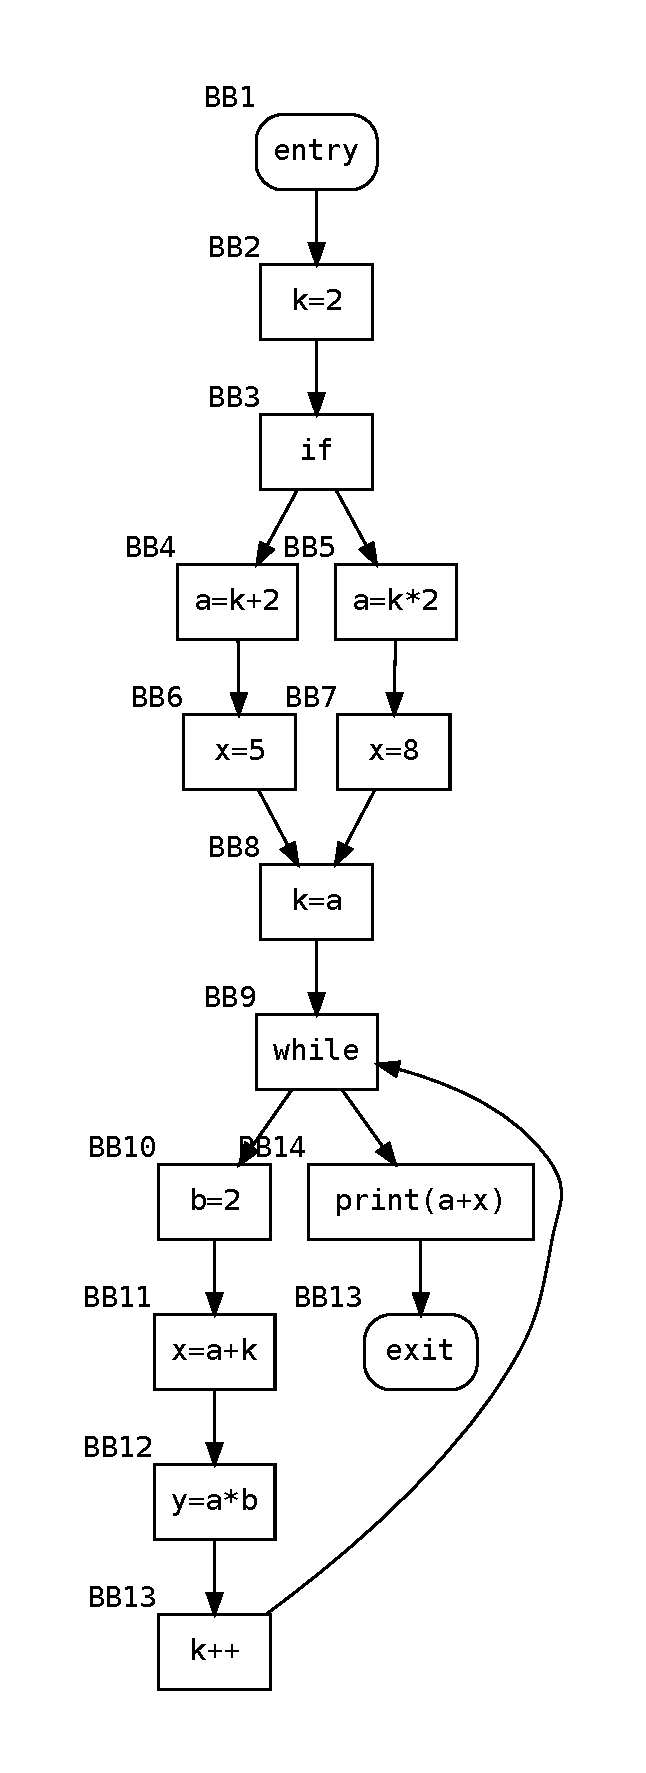
\includegraphics[width=0.45\textwidth]{graphs/constant_propagation.pdf}
	\caption{Constant Propagation example}
	\label{fig:enter-label}
\end{figure}

\begin{table}[H]
	\centering
	\begin{tabular}{|c|c|c|c|c|c|c|}
		\hline
		              & \multicolumn{2}{c|}{\textbf{Iteration 1}}                                 \\ \hline
		              & \textbf{IN[B]}                            & \textbf{OUT[B]}               \\ \hline
		\textbf{BB1}  & $\varnothing$                             & $<k,2>$                       \\ \hline
		\textbf{BB2}  & $\varnothing$                             & $<k,2>$                       \\ \hline
		\textbf{BB3}  & $<k,2>$                                   & $<k,2>$                       \\ \hline
		\textbf{BB4}  & $<k,2>$                                   & $<k,2>, <a, 4>$               \\ \hline
		\textbf{BB5}  & $<k,2>$                                   & $<k,2>, <a, 4>$               \\ \hline
		\textbf{BB6}  & $<k,2>, <a, 4>$                           & $<k,2>, <a, 4>, <x, 5>$       \\ \hline
		\textbf{BB7}  & $<k,2>, <a, 4>$                           & $<k,2>, <a, 4>, <x, 8>$       \\ \hline
		\textbf{BB8}  & $<k,2>, <a, 4>$                           & $<k,4>, <a, 4>$               \\ \hline
		\textbf{BB9}  & $<k,2>, <a, 4>$                           & $<k,2>, <a, 4>$               \\ \hline
		\textbf{BB10} & $<k,4>, <a, 4>$                           & $<k,2>, <a, 4>, <b,2>$        \\ \hline
		\textbf{BB11} & $<k,4>, <a, 4>, <b,2>$                    & $<k,4>, <a, 4>, <b,2>, <x,8>$ \\ \hline
		\textbf{BB12} & \makecell{$<k,4>, <a, 4>,$                                                \\ $<b,2>, <x,8>$}             & \makecell{$<k,2>, <a, 4>,$ \\ $<b,2>, <x,8>, <y,8>$} \\ \hline
		\textbf{BB13} & \makecell{$<k,4>, <a, 4>,$                                                \\  $<b,2>, <x,8>, <y,8>$}       & \makecell{$<k,5>, <a, 4>,$ \\ $<b,2>, <x,8>, <y,8>$} \\ \hline
		\textbf{BB14} & $<k,4>, <a, 4>$                           & $<k,4>, <a, 4>$               \\ \hline
		\textbf{BB15} & $<k,4>, <a, 4>$                           & $<k,4>, <a, 4>$               \\ \hline
	\end{tabular}
	\caption{Constant Propagation Algorithm Execution Table (Iteration 1)}
\end{table}

\begin{table}[H]
	\centering
	\begin{tabular}{|c|c|c|c|c|c|c|}
		\hline
		              & \multicolumn{2}{c|}{\textbf{Iteration 2}}                                 \\ \hline
		              & \textbf{IN[B]}                            & \textbf{OUT[B]}               \\ \hline
		\textbf{BB1}  & $\varnothing$                             & $<k,2>$                       \\ \hline
		\textbf{BB2}  & $\varnothing$                             & $<k,2>$                       \\ \hline
		\textbf{BB3}  & $<k,2>$                                   & $<k,2>$                       \\ \hline
		\textbf{BB4}  & $<k,2>$                                   & $<k,2>, <a, 4>$               \\ \hline
		\textbf{BB5}  & $<k,2>$                                   & $<k,2>, <a, 4>$               \\ \hline
		\textbf{BB6}  & $<k,2>, <a, 4>$                           & $<k,2>, <a, 4>, <x, 5>$       \\ \hline
		\textbf{BB7}  & $<k,2>, <a, 4>$                           & $<k,2>, <a, 4>, <x, 8>$       \\ \hline
		\textbf{BB8}  & $<k,2>, <a, 4>$                           & $<k,4>, <a, 4>$               \\ \hline
		\textbf{BB9}  & $<a, 4>$                                  & $<a, 4>$                      \\ \hline
		\textbf{BB10} & $ <a, 4>$                                 & $<a, 4>, <b,2>$               \\ \hline
		\textbf{BB11} & $ <a, 4>, <b,2>$                          & $<k,8>, <a, 4>, <b,2>$        \\ \hline
		\textbf{BB12} & $<a, 4>, <b,2>$                           & $<a, 4>, <b,2>, <y,8>$        \\ \hline
		\textbf{BB13} & $<a, 4>, <b,2>, <y,8>$                    & $<k,5>, <a, 4>, <b,2>, <y,8>$ \\ \hline
		\textbf{BB14} & $ <a, 4>$                                 & $<a, 4>$                      \\ \hline
		\textbf{BB15} & $ <a, 4>$                                 & $<a, 4>$                      \\ \hline
	\end{tabular}
	\caption{Constant Propagation Algorithm Execution Table (Iteration 2)}
\end{table}

\end{document}
